\section{Сравнительный анализ}

\subsection{Эмпирическое время выполнения}

Для оценки практической производительности оба алгоритма были запущены
на случайных массивах целых чисел различного размера. Каждый эксперимент
повторялся пять раз, результатом являлось среднее время выполнения.
На рисунке~\ref{fig:benchmark} представлены результаты замеров.

\begin{figure}[H]
    \centering
    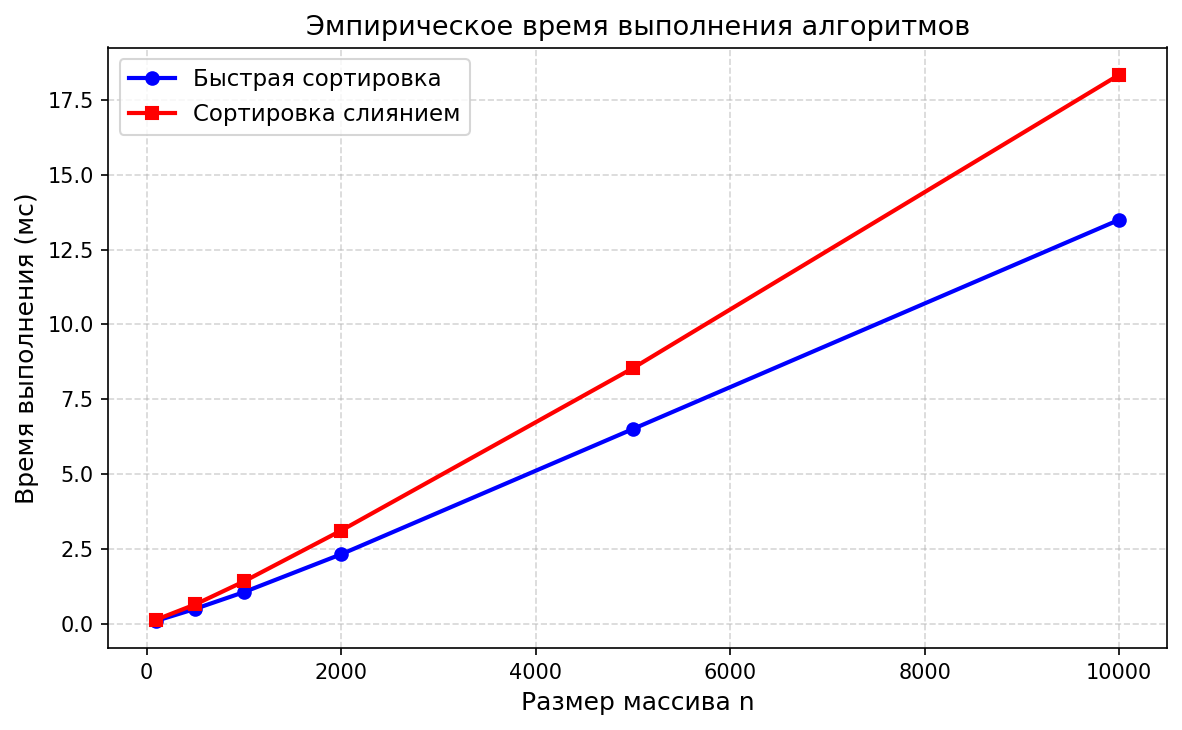
\includegraphics[width=0.85\textwidth]{images/benchmark.png}
    \caption{Эмпирическое время выполнения алгоритмов сортировки}
    \label{fig:benchmark}
\end{figure}

Из рисунка~\ref{fig:benchmark} следует, что на случайных данных быстрая
сортировка незначительно опережает сортировку слиянием за счёт лучшей
кэш"=локальности: операции \mintinline{cpp}{swap} производятся над элементами
самого массива, тогда как \mintinline{python}{merge} создаёт вспомогательные
подмассивы и копирует данные.

\subsection{Использование памяти}

Принципиальное различие алгоритмов"--- потребление дополнительной памяти.
Быстрая сортировка работает \textit{на месте}: единственные накладные
расходы"--- стек вызовов глубиной $O(\log n)$ в среднем случае.
Сортировка слиянием на каждом уровне рекурсии создаёт вспомогательные
массивы суммарным объёмом $O(n)$~\cite{cormen2009}.

Таким образом, для массива из $n$~элементов типа \mintinline{cpp}{int}
(4~байта) суммарный дополнительный расход памяти сортировки слиянием
составит приблизительно:

\begin{equation}
    M(n) = 4n \text{ байт} = \frac{n}{256} \text{ КБ}.
    \label{eq:memory}
\end{equation}

\subsection{Стабильность}

Сортировка слиянием является \textbf{стабильной}: элементы с одинаковыми
ключами сохраняют исходный относительный порядок, что важно, например,
при многоуровневой сортировке таблиц~\cite{merge_analysis}.

Классическая реализация быстрой сортировки \textbf{нестабильна}:
функция \mintinline{cpp}{partition} может нарушать исходный порядок
равных элементов.

\subsection{Итоговое сравнение}

В таблице~\ref{tab:summary} приведено итоговое сравнение характеристик
рассматриваемых алгоритмов.

\begin{table}[H]
    \caption{Итоговое сравнение алгоритмов}
    \label{tab:summary}
    \begin{tabular}{|l|c|c|}
        \hline
        \textbf{Характеристика}    & \textbf{Быстрая сортировка} & \textbf{Сортировка слиянием} \\
        \hline
        Среднее время              & $O(n \log n)$               & $O(n \log n)$                \\
        \hline
        Худшее время               & $O(n^2)$                    & $O(n \log n)$                \\
        \hline
        Доп. память                & $O(\log n)$                 & $O(n)$                       \\
        \hline
        Стабильность               & Нет                         & Да                           \\
        \hline
        Кэш"=локальность           & Высокая                     & Средняя                      \\
        \hline
        Практическая скорость      & Выше на случайных данных    & Стабильна на любых данных    \\
        \hline
    \end{tabular}
\end{table}
